\section{The Models Catalogue Language and Architecture}
 


A software \emph{model} is an abstraction of a software program, which will be instantiated and run using \emph{real data}, software modelling is becoming important for a number of reasons, not least that it enables developers the opportunity to \emph{re-use} code. The Unified Modelling Language UML \cite{UML} or the Eclipse Modelling Framework core \cite{ECORE} ( a subset of UML) are in widespread use for defining and representing software \emph{models}. UML and Ecore are defined at a level which is \emph{more abstract} than the model itself, and one which we term the \emph{meta-modelling} layer. 

The data we have been dealing with in these projects is mostly in the form of textual forms, sometimes in word or PDF format, sometimes in a more specialised form of XML or Excel. The data therefore does have a clear structure, although the clinician running the trial very often has little visibility, knowledge or appreciation of how the data is stored, and who else might in future want to access or manipulate that data.  Although the healthcare providers have work-flows which the patients and doctors follow in the treatment cycle, these are not being considered in this paper.

Sometimes there are standards available governing aspects of the data in question, for instance reporting of a particular clinical trial may need to be in XML which conforms to a particular XSD, however that doesn't mean that the data has been collected with that particular standard in mind.  For the most part clinicians are interested in fairly static data sets, a patient record, the results of a treatment, a clinical trial form, the dynamic aspects are less important, at any rate in terms of the computational representation. What is important is the meaning of the data once it is captured, and in particular how it relates to other data in the same field, for instance is \emph{tumour weight} in one experiment the same as \emph{tumour weight} in another. These two terms may be used in different contexts, for instance prostate cancer and liver cancer, and they may be represented by different values domain in different hospital trusts, for instance one may use grams the other kilograms, the values may be comparable but an adjustment will need to be made to make that comparison.

Thus there are two things we need to identify and reference in building the toolkit, firstly does this \emph{concept} \textbf{mean} the same as that \emph{concept}, and secondly does this \emph{concept} have the same \emph{representation} as that concept. The way in which we can match up concepts in software engineering is by associated them with classes of software objects, and then defining methods which can reference them. 

\subsection{Model Driven Software Development}
......
%%------------NEW STUFF-----------------------%%

%%------------Meta-levels Diagram-----------------------%%


\subsection{Metadata and ISO11179}
ISO11179 is the international standard relating to metadata and in particular metadata registries. It forms the basis of the design of the models catalogue toolkit.

\begin{figure}[here]
	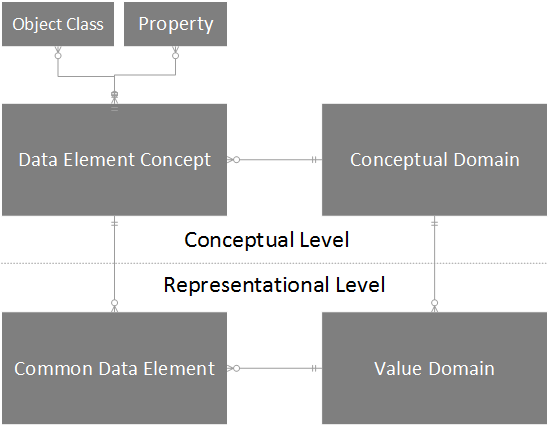
\includegraphics[width=0.48\textwidth,natwidth=610,natheight=642]{BasicISO}
	\caption{Core model for ISO11179 Metadata Registry} 
	\label{fig:basicMDR}
\end{figure}

The ISO11179 standard uses the notion of a \emph{data element concept}, \emph{a data element}, \emph{a value domain}, and a \emph{conceptual domain}. The standard currently confines itself to the detailed level of concepts and data elements and has no notion of collections of data elements or data element concepts, but instead attaches two attributes: an \emph{object class} and a \emph{property} to each data element concept and these attributes allow the data element concept's to be aggregated or classified. This core model of the ISO11179 is illustrated in figure \ref{fig:basicMDR}. The data element concept and conceptual domain entities belong to the \emph{conceptual level}  whilst the common data element and value domain both belong to the \emph{representational level}.


For example an Integer data-type in a programming language may be used to represent inches in a measurement program, it may also be used to count vehicles in a logistics application.  A data element is said to be comprised of a data element concept(DEC) which is its meaning and a value domain(VD) which is its representation.

\begin{table}[h]
	\begin{tabular}{ p{1.8cm} p{2.8cm}  p{3.0cm}  }  % centered columns (2 columns)
		\hline
		Entity & ISO Definition & ISO11179 Implementation Guidelines  \\ 
		\hline
		Data Element Concept(DEC) & An idea that can be represented in the form of a data element, described independently of any particular representation. & A concept that can be represented in the form of a Data Element, described independently of any particular representation.\\
		Common Data Element(CDE) & A unit of data for which the definition, identification, representation, and permissible values are specified by means of a set of attributes. & A unit of data for which the definition, identification, representation and Permissible Values are specified by means of a set of attributes. \\
		Value Domain (VD) & The description of a value meaning. & A description of a Value Meaning. \\
		Conceptual Domain (CD) & A set of valid value meanings, which may be enumerated or expressed via a description.& A set of valid Value Meanings.\\
		\hline
	\end{tabular}
\end{table}

The table lists the definitions of the key entities used in the standard
Conceptual domains comprise sets of value domains, they provide a collection mechanism of \emph{Value Meanings} which provide representation for a particular data element concepts. Data Element Concepts can then be grouped according to their Object Class, or Property, however whilst this works for a system that is focussed entirely on the metadata units, any working software system will need to group the data elements in a structure that is easily transformed into the components such as Classes and Entities that are used in most information systems.   



\subsection{A Language for Enterprise Meta-Modelling and Architecture(LEMMA) }

The ISO11179 specification illustrates different aspects of the standard using UML class diagrams, and we have used these to inform the development of a very simple domain specific language for metadata, which we are calling the \emph{Language for Enterprise Metadata Modelling and Architecture}. The next section gives a description of the language and highlights how it differs from the meta-model outlined in the standard. Probably the key changes are that we have added in containers to handle data element collections, calling these \emph{DataClasses} and to handle collections of these \emph{DataClasses} which we have introduced entities called \emph{DataModels}.

A simplified overview model, without attributes and methods, showing the Ecore model for the LEMMA DSL is shown in Figure \ref{fig:mcSimplifiedOverview}.
%%------------REDO-----------------------%%
\begin{figure}[here]
	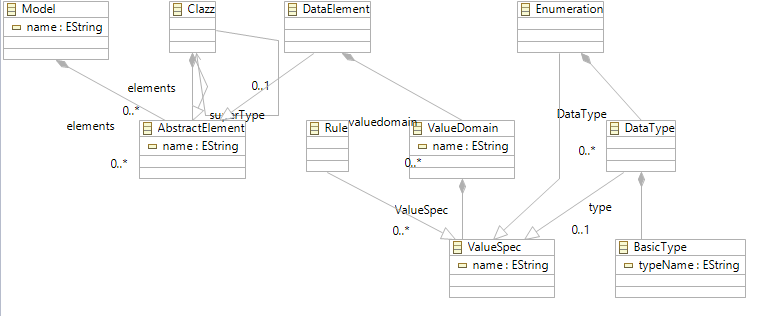
\includegraphics[width=0.5\textwidth,natwidth=610,natheight=642]{ELM_EcoreDiagram}
	\caption{Overview of LEMMA in Ecore} 
	\label{fig:mcSimplifiedOverview}
\end{figure}

\subsubsection{DataModel}
A datamodel is a grouping or containment entity which groups a set of \emph{DataClasses} together. DataModels can be thought of as datasets, or even database schemas, very often in the medical domain they are defined either by XML Schema definition files, or by equivalent schemas written in Excel. 
DataModels are collections of \emph{ConceptElements} which in turn can be either \emph{Data Elements} or \emph{Classes}. There is no real notion of composition or multiplicity, a instance of a DataModel can contain an instance of a Data Element or not as required by the instance.  DataModels are named, have a description and have a version identity.
\subsubsection{DataClass}
A DataClass is a grouping or collection of \emph{attributes} which can be data elements or classes, the attributes are currently \emph{mandatory}, so that DataClass with 5 attributes must have those 5 attributes instantiated in an instance for it to be considered of that DataClass. A dataclass is named to differentiate it from the term \emph{Class} as used in object oriented programming languages, it captures the structural rather than behavioural aspects of a class.  DataClasses represent \emph{Concepts}, and can be \emph{Generalized} into a hierarchy, giving some of the benefits of inheritance to the language.  
\subsection{Data Elements} 
Data Elements can also represent \emph{Concepts} and are by their nature \emph{atomic}.  Each data element is related to a value domain on a one-to-one basis, and the relationship is a two-way relationship.
\subsection{Value Domain}
A Value Domain is the domain in which the data element is represented, it can consist of one or more \emph{ValueSpecs}.
\subsection{ValueSpec}
A \emph{ValueSpec} can be a simple datatype, an enumeration of datatypes, or a rule - such as a regular expression - which defines the way in which a series of characters is formed into a string attribute. 



The original dataset was collected and managed in Excel, as shown in Figure \ref{fig:excelCOSD}

\begin{figure}[here]
	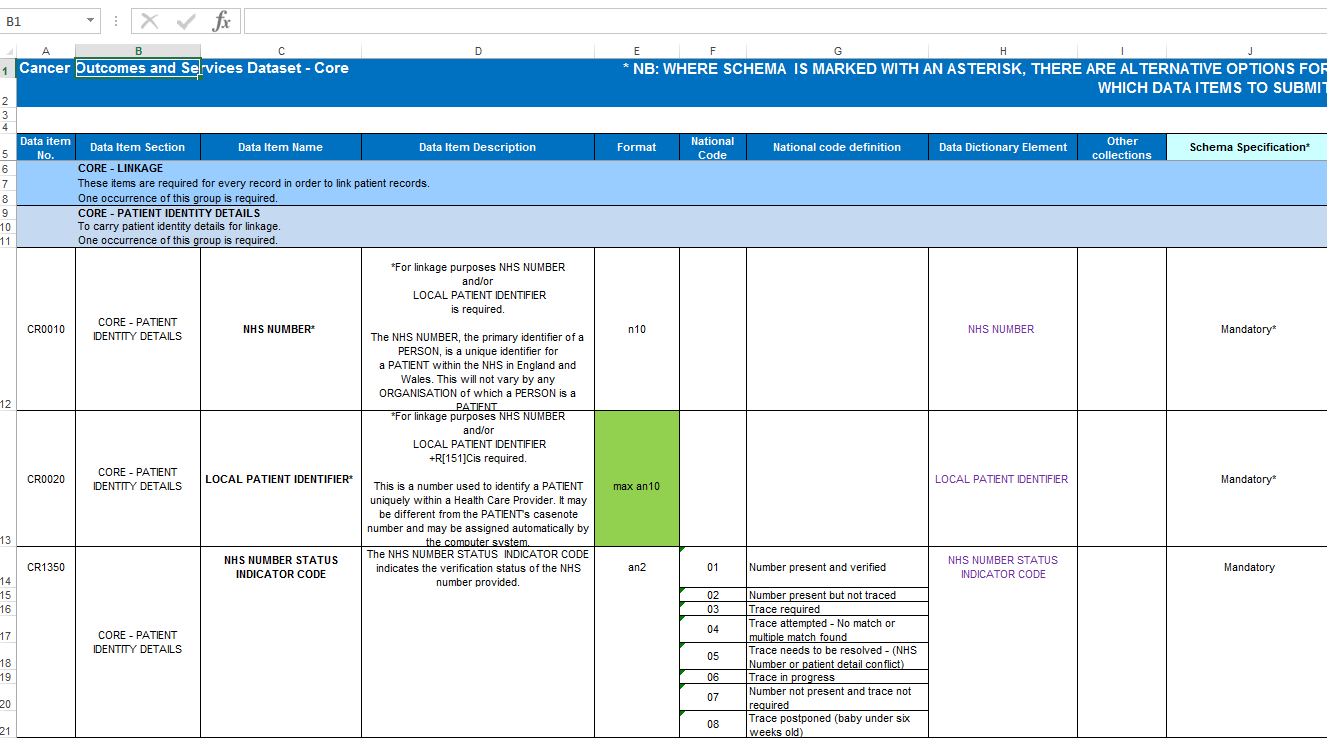
\includegraphics[width=0.5\textwidth,natwidth=610,natheight=642]{COSDExcel}
	\caption{COSD data in Excel Format} 
	\label{fig:excelCOSD}
\end{figure}
The ElmDSL is used to represent a model for Cancer data (part of the Cancer Outcomes and Services Dataset ~\cite{COSD}) in Figure \ref{fig:elmcosd}

\begin{figure}[here]
	\includegraphics[width=0.5\textwidth,natwidth=610,natheight=642]{COSDinLEMMAModel}
	\caption{COSD data in LEMM Model} 
	\label{fig:elmcosd}
\end{figure}



\subsection{Forms and Automatic Software Generation}

%%------------NEW STUFF-----------------------%%

........


